\scanpage{130}%
minaire, - sous réserve tout au plus qu'il existe un tel $E$ sur une extension convenable de $k_x$ (chose peut-être toujours vrai\handwritten{e}).

12. \uline{Exemples instructifs}. Soit $G$ un \deleted{m}monoïde fini. Contrairement au yoga galoisien général, au lieu de prendre $A=k(G)$ (anneau des fonctions sur l'ensemble sous-jacent à $G$) prenons $U=k(G)$, avec l\deleted{a}'application diagonale déduite de $GxG\handwritten{\longrightarrow}G$ (la composition). (On a la bialgèbre ``d\deleted{a}u\deleted{u}ale''\inserted{au sens Cartier} de celle qu'on considère d'habitude). Donc la catégorie $C$ définie par $G$ \deleted{est} peut être considérée comme la catégorie des familles $(\deleted{M}X_g)_{g\ G}$ de vectoriels indexés par $G$, l\deleted{'}e\deleted{application diagonale} produit\inserted{tens.} de deux tels $X$ et $Y$ étant $Z$ défini par $Z_g=\handwritten{\displaystyle\sum}_{g'g''=g}X_{g'}\otimes Y_{g''}$. L'unité est la ``famille de Dirac'' définie par $\deleted{M}X_g=0$ si $g\handwritten{\ne}\deleted{\unsure{0|e}}e$, $\deleted{M}X_e=k$.\inserted{On a une \deleted{\unsure{O|C|c}}Catégorie avec $\otimes,\handwritten{\phi},1$, et de plus un $\handwritten{\unsure{\psi|\mu}}$ si $G$ est commutatif, un $\handwritten{\vee}$ si $G$ est un groupe.}

Un $L$ avec une application diagonale $L\handwritten{\longrightarrow}L\otimes_k L$ compatible avec $U\handwritten{\to}U\otimes_k U$ et donnant un isomorphisme par extensions des anneaux de base, peut s'interpréter comme une famille $(\deleted{M}\handwritten{L}_g)_{g\handwritten{\in}G}$, avec des isomorphismes donnés
\[
(\rlap{\(x\)}-)\qquad \deleted{M}\handwritten{L}_{gg'}\handwritten{\simeq}\deleted{M}\handwritten{L}_g\otimes\deleted{M}\handwritten{L}_{g'}\ .
\]
\margin{Ceci implique que le rang des $\deleted{M}\handwritten{L}_g$ est $0$ ou $1$}
C'est compatible avec $1$ si on a un isomorphisme\inserted{\handwritten{\unsure{(*+)|(**)}}}\handwritten{\begin{tikzpicture}[x=.2cm,y=.2cm,baseline=-.1ex]\draw (0,-.5) .. controls (.2,.1) and (1,.2) .. (1.5,.8);\end{tikzpicture}} $\deleted{M}\handwritten{L}_e\handwritten{\simeq}k$, qui rend\deleted{r}e les isomorphismes $(\rlap{\(x\)}-)$ triviaux quand \deleted{ceux-ci} $g$ ou $g'$ est $=1$. C'est associatif si et seulement si les isomorphismes $(\rlap{\(x\)}-)$ satisfont la \deleted{conditio} conditions d'associativité évidente. De même, $G$ étant commutatif, pour la commutativité. - Le foncteur $F'$ est toujours exact, car $M$ est plat sur $U$.

a) Exemple d'un $\otimes$-foncteur exact, compatible avec $\handwritten{\phi,\psi},1$, \uline{mais non fidèle} (donc pas loc. iso\unsure{\deleted{M}m|\deleted{m}M}. au $\otimes$-foncteur donné). Ce n'est possible dans notre exemple que si $G$ n'est pas un groupe (\deleted{sinon $M$} car $\deleted{M}\handwritten{L}_g$ est de rang $1$ pour $g$ inversible). Mais prenons $G=(e,p)$, avec $p^2=p$, prenons $\deleted{M}\handwritten{L}_e=k$, $\deleted{M}\handwritten{L}_p=0$. On n'a plus le choix pour les isomorphismes $\rlap{\(x\)}-$, qui satisfont toutes les compatibilités (avec $1_x$ par construction, $\handwritten{\phi,\psi}$).
\figure{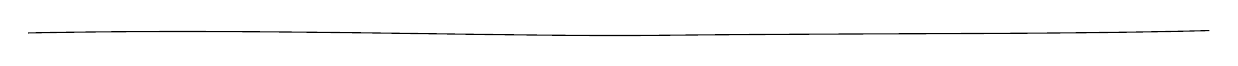
\begin{tikzpicture}[x=1cm,y=1cm]\draw (0,.03) .. controls (3,.09) and (6,-.02) .. (8,0) .. controls (11,.03) and (13,.01) .. (15,.06);\end{tikzpicture}}
\margin{\handwritten{\uline{Question} Un $\otimes$-foncteur \unsure{compatible|comp.tible} avec tout entre $\otimes$-catégories satisfais. à tous les axiomes (y compris rigidité) est-il néc.. fidèle et exact ?!}}
